\documentclass{article}
\usepackage[margin=.5in]{geometry}
\usepackage{graphicx, dblfloatfix}
\usepackage{amsmath, amssymb, amsfonts, mathrsfs, mathtools}
\usepackage[english]{babel}
\usepackage[autostyle, english = american]{csquotes}
\usepackage[normalem]{ulem}
\usepackage[title,titletoc,toc]{appendix}
\usepackage{pgfplotstable}
\usepackage{array, booktabs, colortbl}
\MakeOuterQuote{"}

\pgfplotsset{compat=1.12}


\newcommand{\redchi}{$\tilde{\chi}^2\,$}
\newcommand{\twohalfmf}[2]{$^2 #1_{1/2},\, f = 2,\, m_f = #2$}
\newcommand{\twohalf}[1]{$^2 #1_{1/2},\, f = 2$}
\DeclareMathOperator{\erf}{erf}
\DeclareMathOperator{\cov}{cov}
\DeclarePairedDelimiter\abs{\lvert}{\rvert}%
\DeclarePairedDelimiter{\parens}{\lparen}{\rparen}

\title{Optical Pumping}
\author{Aman LaChapelle}

\begin{document}
\raggedright
\maketitle

\begin{abstract}
  We investigate the effects of an applied external field on Rubidium-87 atoms, known as Zeeman splitting.  We will further investigate the process known as optical pumping, which is used to excite electrons from the \twohalf{S} state to the \twohalf{P} state with the goal of creating a fully pumped state, characterized by a majority of electrons in the \twohalfmf{S}{-2} state.  Using this pumped state and the requrements surrounding its creation, we will further investigate stimulated emission of photons as well as Larmor Precession, which occurs under another special set of circumstances.
\end{abstract}

\tableofcontents
\newpage

\section{Introduction}%%%%%%%%%%%%%%%%%%%%%%%%%%%%%%%%%%%%%%%%%%%%%%%%%%%%%%%%%
  Here we investigate the effects of Zeeman splitting on Rubidium-87 atoms.  More precisely, we investigate the process that is undertaken in order to 'pump' the atoms into an excited state.  There are many uses for such a process, there are certain times when it is simply advantageous to have a macroscopic number of atoms in a single, well-defined state which this process can achieve.  Another possible application is to construct a 3-level system (as opposed to the 2-level system we encounter here) and use that to achieve true population inversion in order to create a laser.

  Returning to the task at hand, we investigate, specifically, properties of the \twohalfmf{S}{-2} state.  Due to thermal fluctuations and the fact that this particular state is an excited state of Rb-87, it is highly unlikely that a macroscopic portion of the atoms will be in that particular state at any given time, so we must find a way to put them there.

  While there exist methods to perform this action - that is, pump Rb-87 into a given state, we perform checks to be certain that they are doing what we expect them to do.  We also take measurements to ensure that we aren't seeing a figment of some other effect and that we are in fact seeing optical pumping of the Rb-87 atoms into the state we have selected.
\section{Theory}%%%%%%%%%%%%%%%%%%%%%%%%%%%%%%%%%%%%%%%%%%%%%%%%%%%%%%%%%%%%%%%
  \subsection{Zeeman Effect}
    The Zeeman effect occurs because of an applied magnetic field onto an atom.  It causes a coupling between the atom's magnetic dipole and the external field, which causes an energy splitting.  The energy perturbation is simple, given by
    \begin{equation*}
      E_z = -\vec{\mu} \cdot \vec{B}.
    \end{equation*}
    This can be simplified, or expanded into a form that depends more obviously on the quantum numbers of the atom like so
    \begin{gather*}
      E_z = g_f \mu_B \abs{\vec{B}} m_f \\
      \mu_B = \frac{e \hbar}{2m_e} \\
      g_f = g_j\frac{f(f+1) + j(j+1) - i(i+1)}{2f(f+1)} \\
      g_j = 1 + \frac{j(j+1) + s(s+1) - \ell(\ell+1)}{2j(j+1)}
    \end{gather*}
    It should be noted that each of these statements depend on the state that the atom is in, but here we take a single value of $g_f$ (and thus $g_j$), and so we can use the following approximation to calculate the energy level separation
    \begin{equation}
      \Delta = (5.79 \times 10^{-9} \, \frac{eV}{G}) g_f \Delta m_f \abs{\vec{B}}.
    \end{equation}

  \subsection{Thermal Noise, Boltzmann and Bose-Einstein Statistics}
    Because there is a certain amount of noise in the energy spectrum simply due to the ambient energy in the room, we must find some way to account for how many atoms are in any given state at any certain time.  Luckily Bose and Einstein built on the foundation of Boltzmann and delivered to us Bose-Einstein statistics to understand the energy distributions of the atoms due to thermal noise.  We can begin from the partition function and write (assuming the atoms do not interact and are indistinguishable)
    \begin{gather*}
      \mathcal{Z} = \sum_j{n_{\epsilon}e^{\frac{\epsilon_j}{k_B T}}} \\
      \text{we introduce}\,\, \beta = \frac{1}{k_B T} \,\, \text{and write}\\
      \mathcal{Z} = \frac{1}{1 - e^{-\beta (\epsilon_j - \mu)}}
    \end{gather*}
    where $\mu$ is the chemical potential attributed to that particular site/atom.  We can, from this, derive the average number of atoms in each state as
    \begin{equation*}
      \bar{N} = \frac{1}{e^{\beta(\epsilon - \mu)} - 1}
    \end{equation*}
    We can find this number, $\bar{N}$ for each of the energy levels in question and describe the system in this way - creating a map of the number of particles in each state versus the energy of each state.  Because of this, we can calculate the ratio of occupations between the \twohalfmf{S}{\pm2} states.  In this example, the $m_f = 2$ state is lower energy.
    \begin{gather*}
      \frac{N_{m_f = -2}}{N_{m_f = 2}} = \frac{N_1}{N_2} = \frac{e^{\beta \Delta_{m_f = -2}} - 1}{e^{\beta \Delta_{m_f = 2}} - 1} \\
      \frac{N_1}{N_2}  = \frac{e^{-2 \beta g_2 \mu_B \abs{\vec{B}}} - 1}{e^{2 \beta g_2 \mu_B \abs{\vec{B}}} - 1} << 1
    \end{gather*}
    From this we can see that there will be a miniscule number of atoms in the excited state, and in general we cannot make definite statements about the state the atoms are in.  However, if we optically pump the atoms into the $m_f = -2$ state, we will see that a macroscopic number of them will be in that state, causing something similar to population inversion.

  \subsection{B-flip, RF De-Pumping and Larmor Precession}
    In order to check if we have achieved a pumped state, we use several techniques to observe characteristics of a pumped optical state - that is the ability to remove it from said state at will with a variety of methods.  The easiest method is to simply flip the $\vec{B}$ field and with that we will see that the atoms de-pump and then return swiftly to a pumped state.  The next way that we can check that we have reached a pumped state is to depump it with an RF field.  What the RF field does is to stimulate emission of photons corresponding to the gap between the pumped $m_f = -2$ state and one of the others.  When we tune the RF field into resonance with this energy gap we will see a depump signal that is triggered at recurring values of the RF field.  This alerts us to the resonance frequency, which we can then fine-tune with trial and error to find an accurate value.  This will tell us, in effect, the splitting between Zeeman levels and allow us to investigate the properties of Zeeman splitting as well as optically pumped atoms in an external field.

    \hspace{.25cm}

    Another way that we can test the effect of Zeeman splitting on these atoms is to cancel as many fields as we can, save for a low frequency, low amplitude rotation (a weak B field changes from the $\hat{x}$ direction to the $\hat{y}$ direction with a frequency of $\approx$0.5 Hz), and then pump the atoms and observe the Larmor precession that occurs just after the depump part of the signal.  What happens is that during the pump cycle, the atoms are aligned to the field in the $\hat{x}$ direction. They then depump, and the field is flipped.  When the field is flipped, the precession cones precess about this new field axis, causing what we know as the Larmor precession.  From observing this we will be able to extract the frequency of the precession and determine the gyromagnetic ratio of Rb-87 as a function of the B field.
\section{Apparatus and Experimental Methods}%%%%%%%%%%%%%%%%%%%%%%%%%%%%%%%%%%%
  The apparatus is rather complicated, and rather than try to render by hand the experimental setup, we will shamelessly steal a picture that the staff of PHYS 21102 have graciously provided for us, Figure~\ref{apparatus}.

  \begin{figure}[!htb]
    \centering
    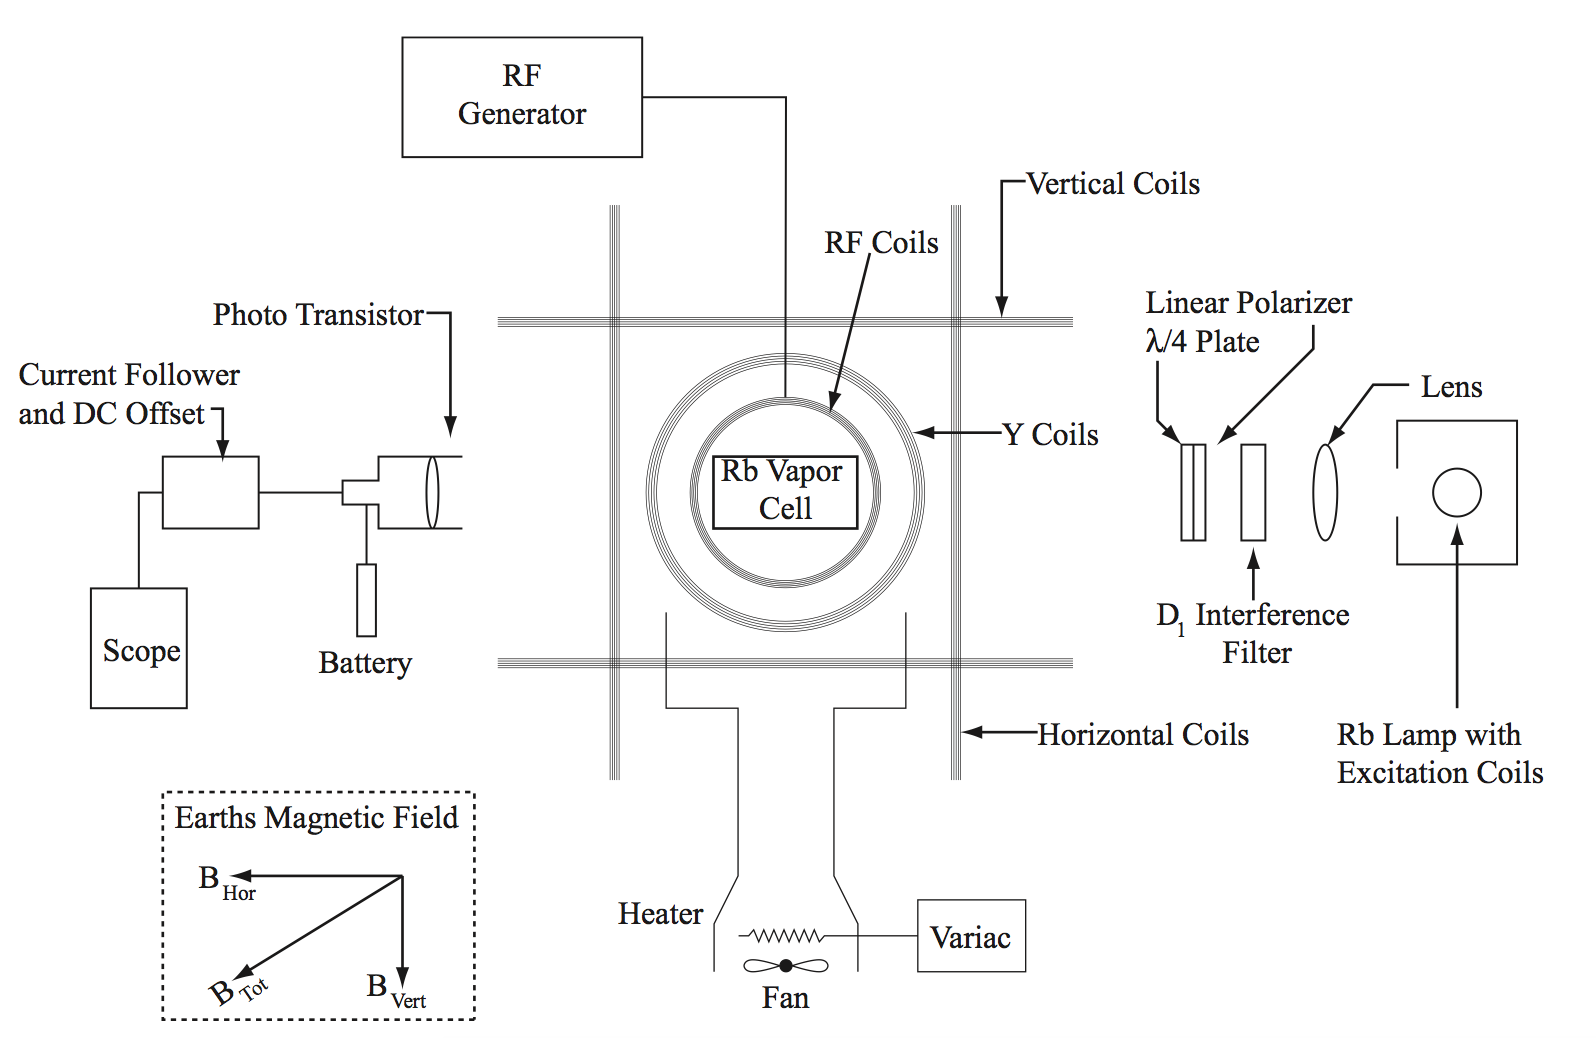
\includegraphics[scale=.25]{apparatus.png}
    \caption{Individual components are labeled, and will be discussed further subsequently.  It should be noted that the Z coils are on top of (share an axis with) the Horizontal coils in the diagram.}
    \label{apparatus}
  \end{figure}

  \begin{figure}[!htb]
    \centering
    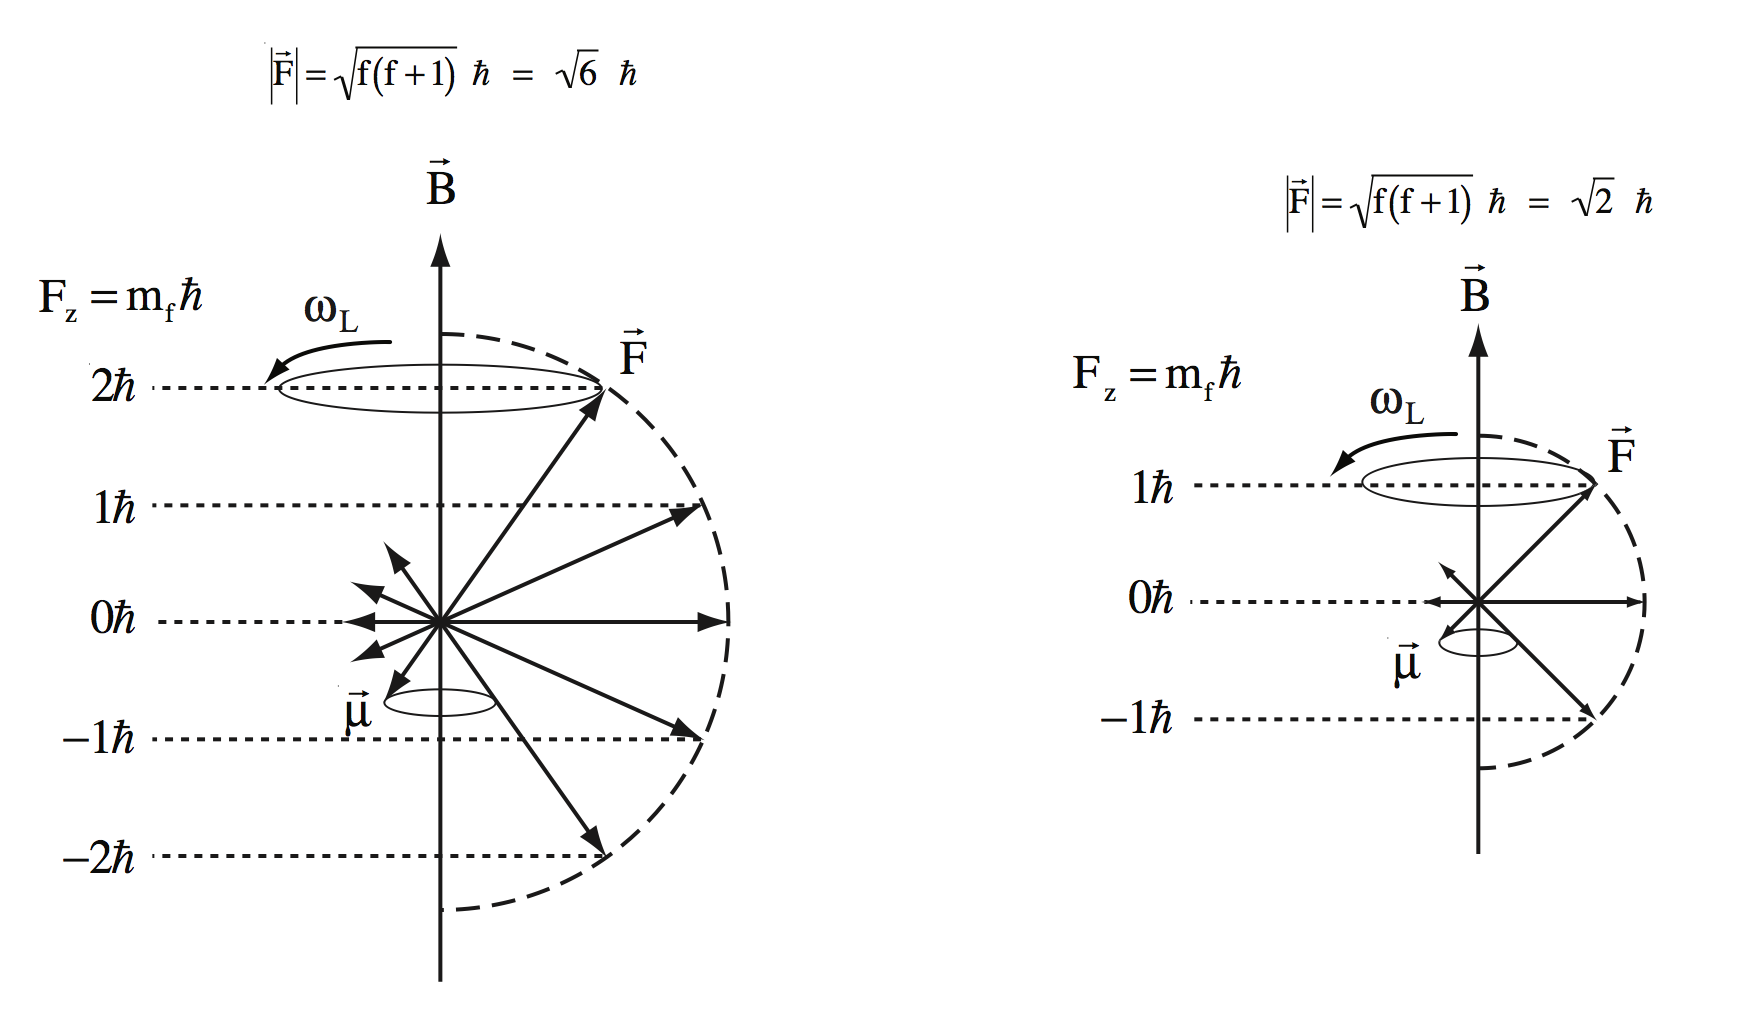
\includegraphics[scale=.25]{cones.png}
    \caption{A model of the precession cones that shows how the conservation of angular momentum causes transitions.}
    \label{cones}
  \end{figure}

  In order of the sequence of events as seen by a photon travelling through the Rubidium cell, the components (grouped) are:
  \begin{itemize}
    \item Rb Lamp
    \begin{itemize}
      \item This gives photons in the general range of the $D_1$ transition, in a wide enough bandwidth that we can excite any of the \twohalf{S} $m_f$ levels.  The goal is to use this light to pump the atoms into the \twohalf{P} state from which they will fall into the \twohalfmf{S}{-2} state.  This is commonly referred to as a $\Lambda$-system due to its shape when drawn on an atomic energy diagram.
      \item The lamp itself contains a Rb bulb with an RF oscillator.  The whole apparatus is kept at an elevated temperature to keep the Rb from solidifying.
    \end{itemize}
    \item Optical components - lens, 1/4 wave plate, and $D_1$ interference filter
    \begin{itemize}
      \item The lens is used to focus the light into the interference filter and the 1/4 wave plate.  The interference filter restricts the light passing through to the wavelength of the required transition, about 780 nm.  Since all the light passing through these optical components is still randomly polarized, we pass it through a linear polarizer combined with a 1/4 wave retardation plate to create a circular polarizer.
      \item The circular polarizer is crucial because the conservation of angular momentum is what favors the transitions (along with the applied $\vec{B}$ field) from lower $m_f$ levels into the higher energy $m_f = -2$ level that we want to investigate.  Figure~\ref{cones}  shows a cartoonish picture of this concept.  The prepared light causes the atoms to jump from a lower energy state into a higher energy state because absorbing the photons necessitates conservation of angular momentum (from the photon spin) and conservation of energy.  The circular polarization ensures that there are only photons of a certain polarization and spin incident upon the Rubidium which causes the asymmetric selection towards the higher energy states.
    \end{itemize}
    \item Helmholtz coils surrounding the Rb vapor cell
    \begin{itemize}
      \item These are used to provide an applied magnetic field.  We will disturb the constancy of this field in order to investigate the properties of optically pumped atoms.  We first simply put square wave pulses through the coils, then later we will use a low frequency (~0.5 Hz) function generator to alternate the current and $\vec{B}$ field to measure the Larmor frequency.
    \end{itemize}
    \item RF Generator
    \begin{itemize}
      \item This is used to de-pump the atoms.  We use this to measure the energy splitting between levels in units of frequency, as well as to check that we have in fact achieved a pumped state.
    \end{itemize}
    \item Heater for Rb cell
    \begin{itemize}
      \item Rubidium is a solid at room temperature.  Due to the fact that there is only very little inside the vapor cell it might not be visible except for a light sheen on the inside of the glass, but it will still cause the experiment to give false results so we elevate the temperature of the cell in order to ensure that all the Rubidium is a gas.
    \end{itemize}
    \item Camera and imaging equipment - photo transistor, current follower/DC offset all attached to the oscilloscope
    \begin{itemize}
      \item The photo transistor turns the intensity of light incident upon it into a voltage.  This signal is transferred through the DC offset to allow us to measure the signal on the scope conveniently, and also to center it to minimize errors due to large offsets.  The scope turns this voltage data into a time-resolved plot that we can examine and understand in the context of the experiment to verify that we at least have a signal that makes sense.
      \item Once the Rubidium atoms are in the pumped state, the transparency of the system will increase greatly due to the fact that no more photons can be absorbed by the Rb-87.  The photodiode and oscilloscope will help us determine in a time-resolved way when the atoms reach their pumped state by showing us when the intensity of light increases to a maximum.  We can likewise identify depumping by watching for when the intensity decreases to a minimum.
    \end{itemize}
  \end{itemize}

\section{Data/Uncertainty Analysis}%%%%%%%%%%%%%%%%%%%%%%%%%%%%%%%%%%%%%%%%%%%%
  \subsection{B Flip}
    We will begin with an example of a scope trace.  On this trace, we have fit the falling exponential of the negative of the pump signal (lower on the plot indicates higher intensity).  This allows us to measure the $\frac{1}{e}$ time with great precision.  The dataset does not, unfortunately, contain enough data points to fit the depump portion as well, but we were able to estimate it on the oscilloscope and so we will report that value.  We know that the higher intensity portion is the pumped state, and that the transition from high to low intensity is the depump cycle, as denoted in the Figure~\ref{trace_example} .
    \begin{figure}[!htb]
      \centering
      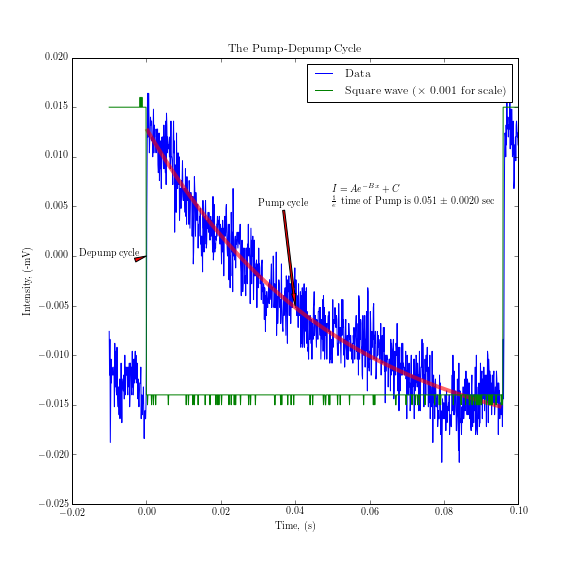
\includegraphics[scale=.65]{../plots/trace_example.png}
      \caption{A plot detailing 1/e time for the pump cycle, as well as simply showing a sample trace.  Error in the 1/e time comes from $\sqrt{\cov(2,2)}$, the diagonal element of the covariance matrix corresponding to the fit parameter multiplied by the argument of the exponential (B in this case).}
      \label{trace_example}
    \end{figure}

    As we can see from the fit, we can measure the characteristic time of the Pump as being $0.051 \, \pm \, 0.020$ sec.  As previously mentioned, we were unable to get enough points on the dataset to properly perform a fit, so we had to estimate the value of the characteristic time for the depump.  We found that that value to be approximately $83 \, \pm \, 9 \, \mu s$.  We notice that as we turn the frequency of the driving wave (a simple square wave) up, it lowers the characteristic pumping time and has very little effect on the depump portion of the cycle.  The reverse is also true, if we turn the frequency of the driving wave down we increase the characteristic time for pumping and still have little effect on the depump portion.  We concluded that the reason this occurs is that there isn't always enough time between cycles to pump the atoms fully, but there is always enough time to depump.

    \hspace{.25cm}

    We can also ensure that we have a pumped state by removing the 1/4 wave plate/polarizer combination.  When we do that, we notice that the intensity goes to zero - since we are no longer filtering the photons they don't have any tendency to shift the atoms to any particular state, i.e. their effects on the atoms are completely random and as such we don't see any atoms pump into an excited state (indicated by a raised intensity).  Of course it's impossible to say that this holds 100\% - there will be some that go to that excited state according to statistical and thermal fluctuations, but the trace that we see is a horizontal line and so we have confidence that it is certainly not a macroscopic number of the atoms.

    \hspace{.25cm}

    One way that we observe the effects of optical pumping was to observe the effects of the Earth's field on the atoms and the whole process.  As can be seen in figure 1, there are components in the vertical and horizontal directions, leading to a net field that points more or less into the floor with a significant component pointing towards magnetic North (slightly north of Wasilla, AK).  Using the helmholtz coils, we can tune the vertical field to exactly cancel the earth's field.  If we use a reduced square wave amplitude, we will notice that during one half cycle the intensity will not change - we will not see pumping during the one half cycle where the applied field points south.  This is because if we point the applied field south such that it exactly cancels the earth's field (which points North), there is no field on the atoms, and thus no Zeeman splitting.  Since there is no splitting, we would not notice any pumping that occurs from a hyperfine state back to itself.  Thus we see a trace like Figure~\ref{reduced}

    \begin{figure}[!htb]
      \centering
      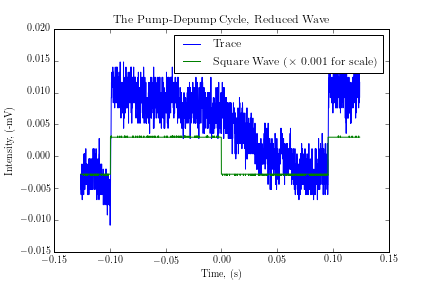
\includegraphics[scale=.75]{../plots/reduced_wave.png}
      \caption{The flat portion corresponds to the part of the cycle where the applied field cancels the earth field and so there is no preferred direction.  The other portion corresponds to normal optical pumping.}
      \label{reduced}
    \end{figure}

    Granted, the flat portion is not entirely flat, but that adjustment is extremely delicate.  We achieved a better example later, but were unable to (due to time constraints) capture the trace, so this is the example that we have.

    \hspace{.25cm}

    The cancellation occured at a horizontal current of $0.18 \pm 0.01$ A (we could vary the current by approx 0.005 A in either direction before we saw a pumping signal).  We can find the $\vec{B}$ field in the north direction as follows:
    \begin{gather*}
      B_{Horiz} = \frac{8 \mu_0 N I}{\sqrt{125} a} \\
      B_{Horiz} = \frac{8 \cdot 1.257\times10{-6} \cdot 36 \cdot 0.18}{\sqrt{125 \cdot 25\times10^{-2}}} = 23.3\times10^{-6} \, T \\
      \frac{\delta B_{Horiz}}{B_{Horiz}} = \sqrt{\parens*{B_{Horiz}\times\frac{\delta I}{I}}^2 + \parens*{\frac{\delta a}{a}}^2} = 20\% \\
      20\%\cdot 23.3\times10^{-6} = 4.7\times10{-7} \\
      B_{Horiz} \pm \delta B_{Horiz} = (23 \pm 5) \times 10^{-6}
    \end{gather*}

    We can calculate the vertical component of the earth's field in much the same way.  When we apply a vertical field of exactly opposite to the earth's field, we will see a completely flat trace.  We turn off the signal generator and sweep the vertical field through the value of the earth's field.  As we reach exactly that value, we will see that there is again no splitting and so no pumping at all.  Keeping the horizontal field cancelled we see a completely flat trace, no features at all.  This occurs at a vertical current of $0.33 \pm 0.01$ A, which corresponds to a field of $B_{Vert} = (460 \pm 14) \times 10^{-7}$ T, using a method analogous to above (the only change is the value of a, the radius of the coil goes from 25cm to 23.5 cm, the absolute uncertainty in that measurement doesn't change, however and the fractional uncertainty changes a miniscule amount that is taken into account appropriately).

    \hspace{.25cm}

    Thus we have come to the conclusion that the Earth's B field has values of:
    \begin{gather*}
      B_{Vert} = (46 \pm 1.4) \times 10^{-6} \, T \\
      B_{Horiz} = (23 \pm 5) \times 10^{-6} \, T
    \end{gather*}
    which compares to the NOAA \cite{NOAA} values of:
    \begin{gather}
      B_{Vert} = 50331.9 \, nT \approx 50.3 \times 10^{-6} \, T \\
      B_{Horiz} = 19098.9 \, nT \approx 19.1 \times 10^{-6} \, T
      \label{NOAA}
    \end{gather}

    For the horizontal field, we were actually within 1$\sigma$ of the NOAA value~(\ref{NOAA}).  This is likely due to our larger uncertainties on the horizontal field calculation - since we used fractional uncertainty and that value was simply smaller.  In the case of the vertical field, we were within 3$\sigma$, which is not terribly accurate.  Given more time, we could have made more measurements but due to time constraint we couldn't.  It is possible that we were thrown off due to other sources in the room, but it would have to be a significant source of field and we are not sure that anything in the room qualifies (aside from the control stack, but that is necessary to the experiment, plus we are dubious as to the strength of that field) as a significant perturbation.  Overall, it was likely just due to the fact that we only had time to perform one measurement, had we been able to take multiple we would have gotten closer.

    \hspace{.25cm}

  \subsection{RF Depumping}
    The primary reason to measure RF depumping was to make a high-precision measurement of the Earth's ambient B field.  Once we had confirmed that we were indeed optically pumping the atoms (yet again) by observing the depump signal, we made high precision measurements of the Earth's B field.

    \begin{figure}[!htb]
      \centering
      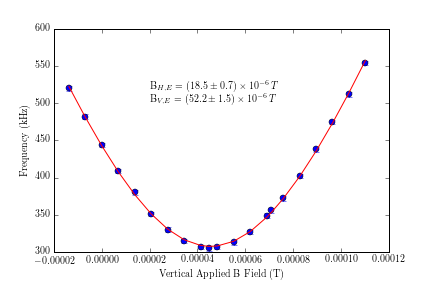
\includegraphics[scale=.7]{../plots/earth_field.png}
      \caption{The fitting for this function was a horrible ordeal, and we will save the reader from trying to understand the goodness of fit measurements in their raw form.  We will interpret and present them in a much clearer form.  We fit to the function $f = \frac{\Delta E}{h}\sqrt{(B_{v,e} - B_{v,app})^2 + (B_{h,e} - B_{h,app})^2}$ with $B_{h,app}$, $\Delta E$ and $h$ fixed, the $B_{\,\,,e}$ as fit parameters, and $B_{v,app}$ as our independent variable.}
      \label{earth_field}
    \end{figure}

    Figure~\ref{earth_field} was the way that we made these high-precision measurements.  Performing the fit was horrifyingly awful, and so let's spend a few moments understanding the fit statistics (as it will help us understand the uncertainties on what seems to be an excellent fit).  The \redchi value was, due to very low uncertainties in the data points, \redchi = $1.27\times10^{3}$, which is absurd.  This prompted a look at the covariance matrix, which also had some absurdly large values, on the order of $10^5$.  As we will do more later, we then decided to perform a fit on simulated data drawn from a normal distribution about each point in order to try and establish the variance in the fit parameters.  This returned values that were exactly half the final values shown on the plot.  However, they were not as stable as we would have liked, and so since the fit was a 2-parameter space, we were able to actually plot the 2-D surface embedded in 3-D that represented the fit parameters, and calculate the Jacobian and Hessian of the points where the fit parameters lie.

    \hspace{.25cm}

    Armed with this information, we determined that it would be an acceptable estimate to simply double the values of the uncertainty we realized in the technique using simulated data.  This was due to some odd flatness in the surface around the minima that corresponded to the best fit that seemed to indicate a sort of valley to a nearby local minimum which could cause issues.  We were not entirely sure that this is a rigorous way to proceed, but it was the best way we could think of.

    \hspace{.25cm}

    As can be seen, the fitted values actually correspond quite well to the values obtained from the NOAA(\ref{NOAA}).  Both of them are within 1$\sigma$ of the literature values, indicating that at we got a value closer to the literature than at least 67\% of measurements, which is an acceptable value.

  \subsection{Larmor Precession}
    The first item of interest for this report in particular is a simple plot of the larmor precession itself.  We will see that, in particular, we can fit the sine curve and extract the frequency this way.  Choose for example Figure~\ref{sinwave} , taken at 0.055A (Vertical Helmholtz coils).

    \begin{figure}[!htb]
      \centering
      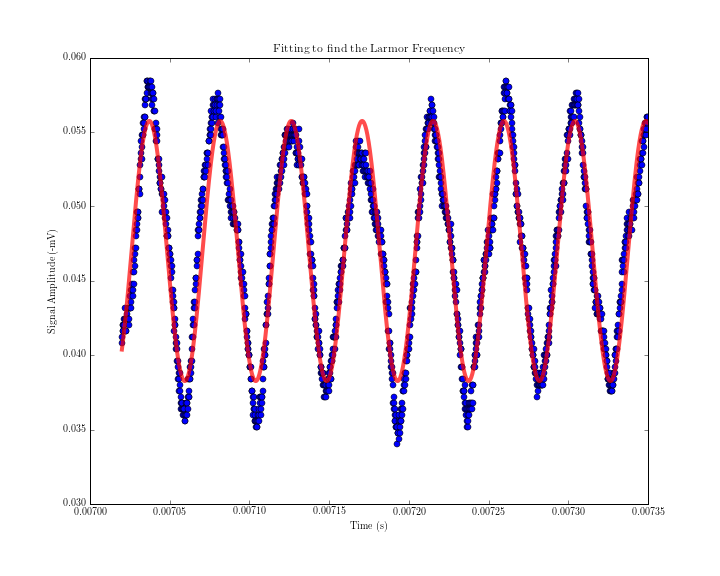
\includegraphics[scale=.45]{../plots/(larmor_y0_055A).png}
      \caption{The red line corresponds to the fitted curve.  The curve parameters are not shown because they are not particularly enlightening, nor do they fit on the axes in an aesthetically pleasing way.}
      \label{sinwave}
    \end{figure}

    In Figure~\ref{sinwave} we fit a curve of the form
    \begin{equation*}
      A\sin(\omega t + \delta) + B.
    \end{equation*}
    This is not completely correct, as the larmor precession is suppressed due to the fact that the precession of the atom itself, the $m_f$ precession aligns to the new field.  However, in order to extract a frequency, we need only fit a few periods to extract a good value for the frequency, as we have done here.

    \hspace{.25cm}

    In Figure~\ref{sinwave} , we see that the fit is actually quite good, and so we can have good confidence in the values of the frequency extracted.  If we wish to increase our confidence, we can take a normal distribution of data around each point, and pick a random point within that distribution at each point.  We then fit that simulated data and take the standard deviation of those fit values to extract uncertainty.  This leads to good certainty in our fit values like this:
    \begin{equation}
      f \pm \delta f = (141210 \pm 70) Hz
      \label{freq_sample}
    \end{equation}
    We have good confidence in our fit values and do believe that they are representative of what we measured.

    We can from this extract values for the frequency of larmor precession and plot these values versus the value of the vertical field at that frequency in order to find the gyromagnetic ratio.

    \begin{figure}[!htb]
      \centering
      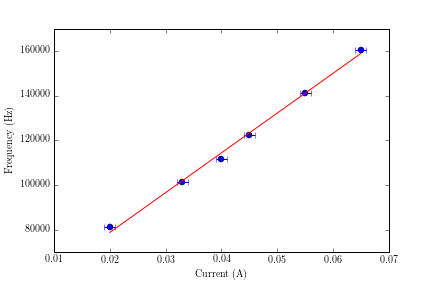
\includegraphics[scale=.5]{../plots/gyromagnetic_ratio_fit.png}
      \caption{Fitting to find the gyromagnetic ratio.  Values that we can compare against fluctuate, but most agree on a value between 6.7 GHz/T and 7 GHz/T.}
      \label{gyromagnetic}
    \end{figure}

    Looking at Figure~\ref{gyromagnetic}, we notice a few things.  The first is that the \redchi value is absurdly high.  I would direct attention to the sample of our frequency data (eq~\ref{freq_sample}) and say that since our uncertainty is so incredibly low (on the order of 0.06\%) the \redchi is not a good parameter for determining goodness of fit.

    \hspace{.25cm}

    Here again, we used a rather interesting technique (as for the sine wave above Figure~\ref{sinwave}) for which we will go into more detail here.  For each point, we use the estimated error on that point as the standard deviation of a normal distribution centered at our best guess value.  From that normal distribution, we use the numpy random functions to pick a random value within that distribution.  Once we've suitably randomized some simulated data, we fit to that simulated data.  Then we repeat this process (in this case, 5000 times) and record all the fit parameters.  We then assume that those fit parameters are normally distributed, and take the standard deviation of those fit parameters as the error in our fit.  If we were to take the standard deviation of the mean instead of the standard deviation, we would get a much smaller uncertainty, but that is not necessarily correct due to error in the x coordinate (in this case the B field).  Thus we pick the value that best represents the error of our dataset, and furthermore is independent of the number of iterations of this process (because then we could artificially deflate the uncertainty in the fit).

    \hspace{.25cm}

    If we now compare our fitted value to the values that we managed to find from others who have performed this experiment around the world (whose results range from 6.7 to 7 GHz/T), we can calculate our confidence in our value.  Our value was within 2$\sigma$ of the low end of the 'literature' range, and within 3$\sigma$ of the top end.  This is not particularly spectacular, which indicates that there is some sort of external uncertainty that is coloring our data.  However, as we saw before, it is unclear what is causing this uncertainty, and as such we cannot find it without performing multiple trials, where we set up the experiment from scratch and then perform the measurement a few times.  Due to time constraints we cannot perform such a feat, but that would be the only way to actually understand the source of our uncertainty.

    \hspace{.25cm}

    We can now take our value of the gyromagnetic ratio and calculate the expected Larmor precession frequency at a high field.  This is a simple calculation, shown below.  We need a few pieces of information - we will choose a value of the B field from the RF depumping section and the corresponding frequency.  The point we will try will be the minimum of Figure~\ref{earth_field}
    \begin{gather*}
      B_{tot} = \sqrt{\parens*{B_{H,E} - B_{H, App}}^2 + \parens*{B_{V, E} - B_{V, App}}^2} \\
      B_{tot} = \sqrt{(23.183\times10^{-6}-18.5\times{10^{-6}})^2+(52.2\times10^{-6}-52.2\times10^{-6})^2} = 4.6\times10^{-6} \, T \\
      \gamma \cdot B_{tot} = 275.1 \pm 15 \, kHz = f_{Larmor} \\
      \gamma_{lit} \cdot B_{tot} = 6.7 \cdot B_{tot} = 308 \, kHz \\
      f_{measured} = 305 kHz \\
    \end{gather*}

    What we see is that the two values, the expected Larmor frequency and the RF frequency are quite close.  This tells us that it is very likely that the same mechanism causes both effects, the RF depumping and the Larmor oscillations.  However, this also tells us that the linear function that we fit to for the Larmor precesison does not necessarily extend.  It is also very possible that that line does extend, we simply did not see it because our value for $\gamma$ was off.  As such, we performed the calculation again using our value for the B field and using the literature $\gamma$, which gives us (at the closest, $\gamma = 6.7 \, GHz/T$) 308 kHz, and at the furthest ($\gamma = 7 \, GHz/T$) 320 kHz.  This means that it is quite possible that the line extends up to even the high field used for the RF depumping portion of the experiment, but we cannot assume and so we must check somehow.  Given more time, a network analyzer and a better oscilloscope we might be able to attempt to fill in the intermediate values of resonant frequency, but alas, time and funds were in short supply.


\section{Conclusion}%%%%%%%%%%%%%%%%%%%%%%%%%%%%%%%%%%%%%%%%%%%%%%%%%%%%%%%%%%%
  In conclusion, most of the experiment was greatly hampered by the fact that we simply did not have enough time.  Had we been given more time we would have performed each section multiple times, which would have allowed us to pinpoint sources of error in our methods.  Even if multiple repititions hadn't allowed us to see the error, we could have seen that multiple values were inaccurate and that would have allowed us to search for some systematic uncertainty.

  \hspace{.25cm}

  We had one successful run, however - the values we extracted for the Earth's field from the RF depump section were quite close to the literature values, which goes to show that the more automation we can insert into a method, the more accuracy we can extract from the system.
\begin{thebibliography}{10}
  \bibitem{NOAA}
    NOAA Magnetic Field Calculators. \\ http://www.ngdc.noaa.gov/geomag-web/\#igrfwmm

  \bibitem{lab manual}
  	University of Chicago Department of Physics. "Introductory Lab: Gamma Cross Sections"\\
  	https://wiki.uchicago.edu/display/P211manuals/Introductory+Lab\%3A+Gamma+Cross+Sections. (Accessed Nov 8-16, 2015)

  \bibitem{taylor}
  	Taylor, John. \emph{An Introduction to Error Analysis}. Sausalito: University Science Books, 1997.
\end{thebibliography}

\end{document}
